\begin{figure}[h]
	\centering
	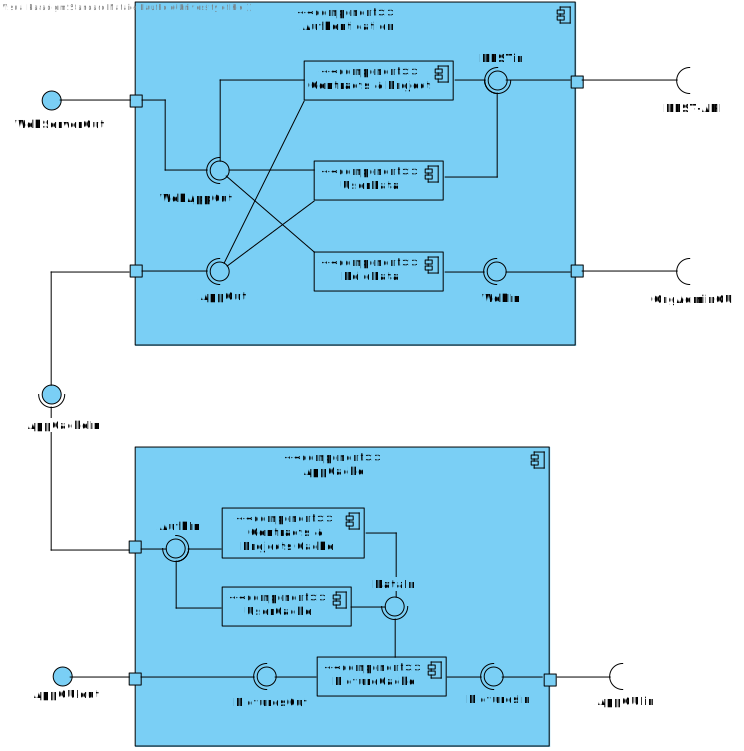
\includegraphics[width=16cm]{img/diagrams/cp_backend.pdf}	
	\caption{Komponentendiagramm - Backend}
	\label{fig:komponentendiagramm-backend}
\end{figure}

\begin{figure}[h]
	\centering
	\includegraphics[width=16cm]{img/diagrams/Component-WebServer.pdf}	
	\caption{Komponentendiagramm - WebServer}
	\label{fig:komponentendiagramm-webserver}
\end{figure}

\begin{figure}[h]
	\centering
	\includegraphics[width=16cm]{img/diagrams/Component-App.pdf}	
	\caption{Komponentendiagramm - App}
	\label{fig:komponentendiagramm-app}
\end{figure}

\begin{tcolorbox}
Die strukturelle Übersicht des zu entwickelnden Systems wird mittels Komponentendiagrammen modelliert. 
Auf jedes Diagramm muss eine textuelle Beschreibung (Fließtext mit Umbrüchen / Absätzen oder Tabelle) folgen, in der die Aufgaben der Subkomponenten beschrieben werden. 
\end{tcolorbox}